\documentclass{MX2020}

\usepackage{lipsum} 
\usepackage{multicol}
\usepackage{cuted}% for environment `strip`
\usepackage{graphicx,float}
\usepackage{caption}
%\usepackage[utf8]{inputenc}
\usepackage[english]{babel}
%===============================================================================

\title{ \bf Implementation of Densely Connected CNN with Multi-scale Feature Attention for Text Classification}
\author{Vishnu Chirukandath Ramesh 1921535
\vspace*{-50pt}}
\usepackage[colorlinks=true,citecolor=blue,linkcolor=blue]{hyperref}
\begin{document}

\MXabstract{Feature selection has a major role to play in the performance of a deep learning process, especially in the case of natural language processing we have to deal with meaning, emotion and, many other complicated characteristics. This work is the realisation of the mechanism to choose variable length features, which is crucial to significantly improve the performance. The normal n-gram will split the data into fixed sized features, in some scenarios it won't work well. sometimes we will get the opposite result also, especially in the case of sentimental analysis and other related fields. There are so many experiments going around the world in search of a good attention mechanism. The densely connected neural network has been a hot topic for a while and has also proven to be highly efficient. Therefore, this implementation makes use of the densely connected structure for the multi-scaled features attention. This work will be tested against the real and fake news data-set available in kaggle.}
{Densely connected convolutional neural networks, Multi-scale feature attention, News classification}

\section{Introduction}
Natural language processing, one of the major areas of application for deep learning algorithm have to deal with many cases including text classification. Deep learning model such as Recurrent Neural Networks (RNN), recursive autoencoders have been commonly used for NLP tasks, specifically Convolutional Neural Network [CNN] has proven to be very successful in computer vision and Text Classification  \cite{Kim,Blunsom,Lei,Zhang,Conneau}.
\newline
Since, Most of the CNN Models make use of convolution filters of fixed size window which can only extract fixed-size n-gram \cite{Zhang,Conneau,Wang} features as a drawback it does not extract variable size features such as, {\textit{phrases}} for better representation\cite{ZhangT}. The issue we may have to face is {\bf{the inability to adaptively select
multi-scale features in a CNN model for text classification.}} Multi-scale features refers ton-gram features with variable {\textit{n}}, such as unigram ({\textit{n}} = 1), bigram ({\textit{n}} = 2), trigram ({\textit{n}} = 3) and so on. For instance, Sentiment classification for sentence - {\textit{“He’s nice to talk to without being patronizing”}} (as shown in Figure1) requires an extraction of unigram feature {\textit{"nice"}} and a trigram feature {\textit{"without being patronizing"}}, which are both positive words or phrases. As shown in figure \ref{fig:intro}, applying size 1 filter results in one positive and one negative feature, meanwhile size 3 filter puts out an ideal (positive phrase) neural response for phrase {\textit{“without being patronizing”}} indicating the unigram response {\textit{"nice"}} is undesirably decreased as the model includes unnecessary information in either {\textit{“He’s nice to”}} or {\textit{“nice to talk”}}.
\newline
An effective approach would be to apply multiple filters with variable window sizes to extract multi-scale features, but even with a large amount of experimental efforts to 
\begin{figure}[h]
    \centering
    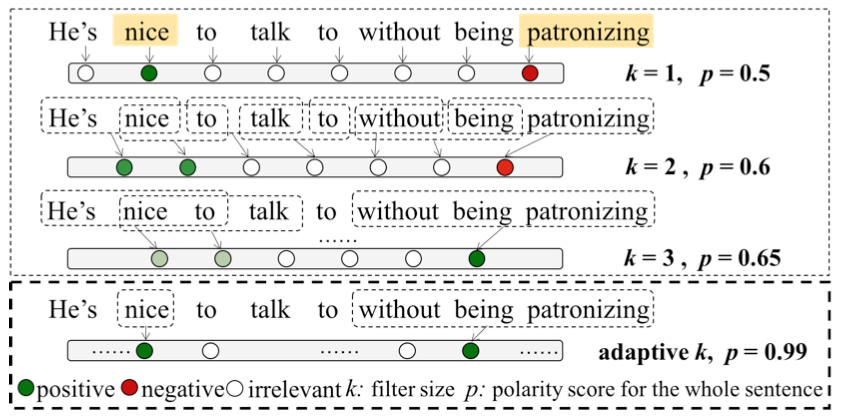
\includegraphics[width=0.5\textwidth]{intro.png}
    \caption{An example illustrating importance of multi scaled feature attention. \cite{Shiyao}}
    \label{fig:intro}
\end{figure}

find optimal combinations of different filter sizes this approach will require learning of several separate, disconnected networks in parallel without exploiting the feature maps from different filter sizes. Therefore, Authors in study \cite{Shiyao} believe in deeper model which can create an hierarchical representations by multi-level abstraction and eliminating the need to re-learn redundant feature maps. As shown in figure 2, the model can create trigram features in third layer (e.g.\(f'(x_1, x_2, x_3)\) ).
by stacking another layer of window size 2 followed by a 

\begin{figure*}
    \centering
        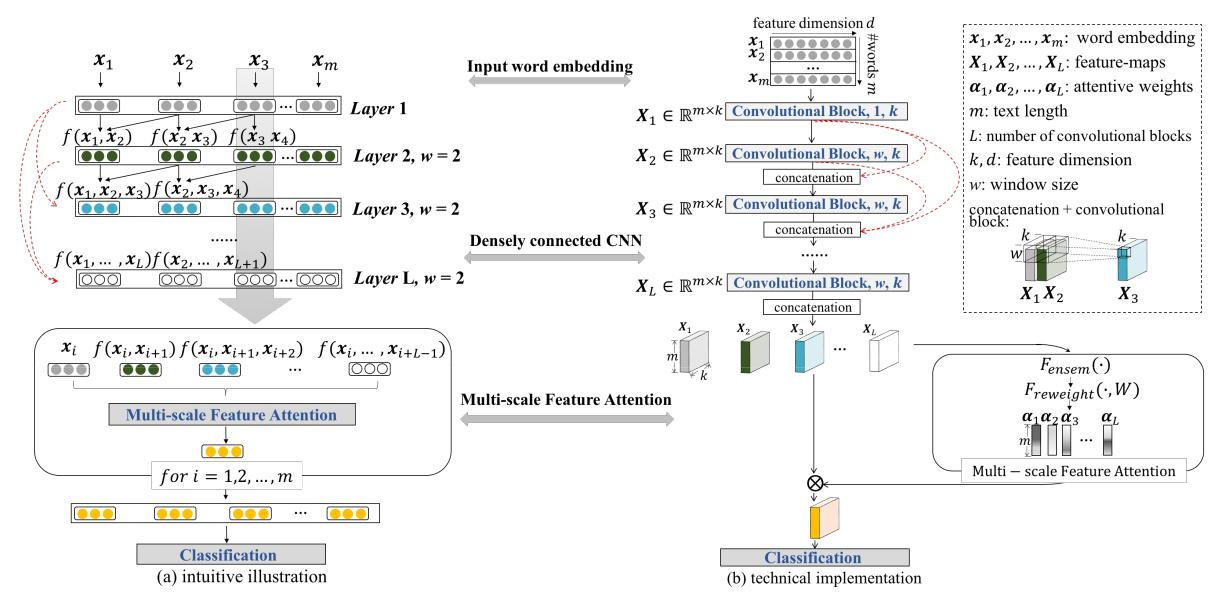
\includegraphics[width=1\textwidth]{model.png}
        \caption{{This picture indicate the the Densely connected CNN with multi scale feature attention. The figure (a) Indicates how the model generate the multi scale features and how the features are used for classification. (b) Technical implementation all the convolution and concatenation operation, dense connection and multi scale feature attention.}}
        \label{fig:model}
\end{figure*}

layer with window size 1. With the dense connection it will be able to make use of the data of the layer above. To select the task friendly feature from all the possible multi scale features, we design attention module before the classification layer. In summary this will implement the Densely connected CNN with multi-scale feature attention for text classification\cite{Shiyao} and test against the real and fake news data-set.

\section{Related Work}
Several noticeable advancement can be noticed in the models for the natural language processing. The Recurrent neural network, including Long short term memory and gathered recurrent unit stated to use widely in the text processing. several other variants are also proposed like \cite{2017b}. The CNN is another most widely used model, the convolution filters on sliding window for next sequence and applied a max operation to capture most useful feature. \cite{Kim} adopted multiple filters with different window sizes to extract multi- scale convolutional features for text classification. A dynamic k-max pooling mechanism was proposed in \cite{Blunsom}. aother proposal is a novel feature mapping 
operator to generate non consecutive n-gram features \cite{Lei}. \par
Several advancement can be seen in the attention mechanisms also, if we equip the neural network models like CNN and RNN, its very likely to get good performance. Among the proposed attention mechanisms, main noticeable are Soft and hard attention \cite{xu} and local and global attention like that list will progress
\section{Method}
The model we are making use is the one mentioned in \cite{Shiyao}. The figure \ref{fig:model} we can find more detailed technical view on the right, and the one on the right it emphasis on the overall view. The inputs to the model begins with text input \( x_0 x_1 x_2 x_3\) and generates multi scale features by convolution blocks with dense connections. The convolution block on the top will generate small gram and the one on downstream ones for large n-grams. The upstream blocks, downstream blocks gets the flexibility with the dense connection, as the the downstream blocks have access to all the upstream blocks. With the attention mechanism, the feature maps will re-weighted with filter ensemble and scale re weight. \[ X = [ x_0, x_1, x_2, ...., x_n]_m_\times_d \] In this case m is the number of words in the text. The output of each layer can be can be be represented as  \( X_l = [ x_l_1, x_l_2, x_l_3, ...., x_l_m]_m_\times_k \). Where \(l\) is the layer index it can be  \(l\) $\leq$ \(L\),  \(L\) is number of blocks convolution blocks and \(k\) is the dimension of the transformed feature representation.
\newline
Each convolution block \(X_l\) which is the function composition of three cascaded operations: a convolution, a back normalization and rectified linear unit (\(X_l = f(W_l, X_l_-_1)\))\cite{nair}. Each \(X_l\) depends on the previous feature \(X_l_-_1\) and the learn able weights \(W_l\), its weight consist of \(k\) filters with size \(w \times k\). Normally in traditional Convolution block use to form a sequential hierarchy, but in this model we follow a dense connection\cite{2017a}. With the dense connection, for a layer \(l\) can make use of all inputs and outputs of upstream layers.\[X_l = f(W_l, [X_1. X_2, ....., X_l_-_1])\] Even though the effective use of these feature is really a key issue.In order to make use of these features for classification the multi-scale feature attention mechanism is useful which will adaptive selects feature of different size \cite{Shiyao}. This mechanism contains two operators: \textbf{filter ensemble} and \textbf{scale reweight}.
\newline
Filter ensemble aims to develop scalar descriptors \(s_l^i\) to represent feature at each scale. This will be later make use of this description during scalar reweigh. \[s_l^i = F_{ensem}(x_l^i) = \sum_{j=1}^{k} x_l^i(j)\]
\newline
\textbf{scale reweight}, it will make use of the descriptor developed with filter ensemble as the input to generate attention weights to re weigh the features. So the final representation \[x_{atten} ^i = \sum_{l=1}^{L} \alpha_l^i x_l^i \] \[\sum_{l=1}^{L} \alpha_l^i = 1, 1 \leq i \leq m \cite{Shiyao}\]

The attention module will pass the re weighted feature map into the classification layer, which has the training objective to minimize the cross entropy loss: \[\phi = \mathcal{L}(y,h(W, X_{atten}))\]
where \(\mathcal{L}(y,h(W, X_{atten}))\) is the predicted output distribution, and y is the referenced distribution. 

\vspace*{10pt}
\section{Experiments}

\subsection{Implementation details}
We have evaluated the model mentioned in the \cite{Shiyao} with the real and fake news dataset. The dataset is available in kaggle. So our data set will have 2 classes one the news is valid and the news is invalid. The dataset will be available like in diffenet file we should combine them and process and shuffle. 
We have used the Glove word embedding was of size 300. Input text is padded into a fixed size as mentioned like in the above table. we used 100 in our case. We used tensorflow V2 for implementing this model.In \cite{Shiyao} the model was implemented with caffe. Now the caffe 2 is a part of Pytorch. we used 5 convultional blocks,  window size \(w\) = 3 and the feature size 128. 
The classification have fully connected MLP with ReLu activation function and softmax output. We used Nadam optimizer with low learning rate. 
\subsection{Main Results}
The model was trained successfully with an accuracy more than 95 percentage and loss around 0.1 on validation set  in 50 epoch. The output graph can be seen in the figures \ref{fig:accuracy} \ref{fig:loss}. When we analyse we can see model started with initial accuracy around 50 percentage and loss about 0.9. and then it started to under fit and again aligned around epoch 34. after 30 the model started to over fit, the validation accuracy started to increase. So the best modal would be around epoch 34.
\begin{figure}[h]
    \centering
    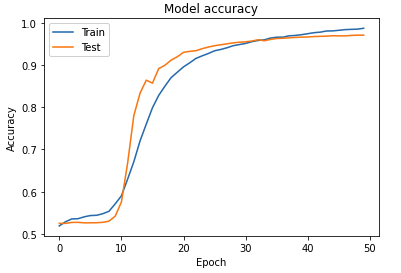
\includegraphics[width=0.5\textwidth]{accuracy.png}
    \caption{Model accuracy for the training with real and fake news dataset.}
    \label{fig:accuracy}
\end{figure}
\begin{figure}[h]
    \centering
    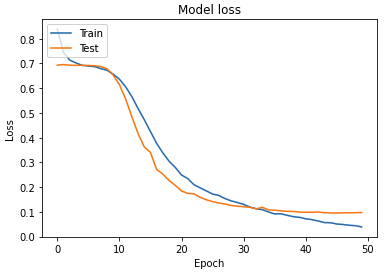
\includegraphics[width=0.5\textwidth]{loss.png}
    \caption{Model loss for the training with real and fake news dataset.}
    \label{fig:loss}
\end{figure}
\subsection{Hyper parameter tuning}
The accuracy and loss is observed with the change of the parameters like learning rate, window size and schedule decay.  There was significant change in the performance 
when changing these parameters. when the window size is reduced to 1 and 2 the performance decreased compared to what we have with window size 3. in the case if learning rate the model was finding local mini-ma at the beginning so the lower learning rate chosen. schedule decay is also we chooses a medium range value to maintain good performance.

\vspace*{10pt}

\section{Conclusion}

The Densely Connected CNN with Multi-scale Feature Attention for Text Classification is a remarkable work. Even though the feature attention mechanism stated to show its significance a while ago with the densely connection and functions made them more power full and more accurate. The data set showed its significance in 6 benchmark data set includes agnews, yelp etc. It gave a significant performance for the data set the we choose which includes data about real and fake news. The model have several layers, it was implemented with caffe by the authors, which was a real power full framework, and it combined with pytorch. In current implementation Tensorflow was the choice, the lack group convolution feature made to think about pytorch but the concatenation process was little complicated in that, so proceeded with tensor flow by implementing group convolution by tensors.
So it increased the number of layers in our model. Overall this model is perfect fit for most of the natural language processing applications.
\vspace*{20pt}

%bibliography
	\bibliographystyle{plain}
	\bibliography{biblio}

\end{document}